\documentclass[11pt]{article}

% Codificación y fuentes
\usepackage[utf8]{inputenc}
\usepackage[T1]{fontenc}
\usepackage[spanish]{babel}

% Geometría
\usepackage[margin=2.4cm]{geometry}

% Matemáticas
\usepackage{amsmath}
\usepackage{amssymb}

% Gráficos
\usepackage{graphicx}
\graphicspath{{figuras/}}

% Tablas
\usepackage{booktabs}
\usepackage{multirow}

% Flotantes
\usepackage{float}

% Hipervínculos
\usepackage{hyperref}
\hypersetup{
    colorlinks=true,
    linkcolor=blue,
    citecolor=blue,
    urlcolor=blue
}

% -------------------------------------------------------
\title{%
    \textbf{Sistema de Memoria Transactiva Multi-Agente}\\
    \textbf{sobre Memorias Asociativas Entrópicas}\\[0.4em]
    \large Reporte Técnico Breve
}
\author{Gabriel Gonzalez\\[0.3em]
\small Directora: Karla Miroslava Olmos Sánchez}
\date{Junio 2026}

% -------------------------------------------------------
\begin{document}

\maketitle

\begin{abstract}
Este documento presenta el sistema EAM-TMS: un sistema de memoria transactiva
multi-agente construido con EAM \cite{pineda2021entropic,pineda2024hetero},
sin gradientes ni retropropagación.
Tres agentes especialistas trabajan sobre ETH-80 \cite{leibe2003eth80}: uno
para \textit{apple}, uno para \textit{horse} y uno para \textit{car}.
Junto con el mediador inicial (TME), reproducen los tres mecanismos de la
Memoria Transactiva de Wegner \cite{wegner1987transactive}.
El sistema alcanza una precisión madura del 98.75\,\% con rechazo claro de lo
que no conoce, y el directorio transactivo se forma en tan solo 13 interacciones
cuando la exposición es variada.
El documento completo desarrolla la teoría, la metodología y los cinco bloques
experimentales.
\end{abstract}

% -------------------------------------------------------
\section{Memoria transactiva de Wegner}

Cuando un grupo de personas trabaja de manera coordinada durante el tiempo
suficiente, el grupo recuerda más de lo que cualquiera de sus miembros podría
recordar de forma individual.
Wegner \cite{wegner1987transactive} llamó a este fenómeno \textbf{memoria
transactiva}: cada individuo mantiene no solo sus propios conocimientos, sino
también un \emph{directorio} de quién dentro del grupo sabe más de cada
dominio.
Cuando un miembro necesita información fuera de su área, consulta ese
directorio, determina a quién preguntar y delega la recuperación.

El modelo identifica tres procesos: la \emph{actualización del directorio}
(tras cada interacción, todos los miembros, incluso los que no respondieron,
registran quién supo responder), la \emph{asignación de información} (lo nuevo
se envía al especialista) y la \emph{coordinación de recuperación} (las
consultas viajan directamente al agente que sabe del tema, sin intermediario).
La transición de una \textbf{fase temprana} mediada a una \textbf{fase madura}
punto a punto es la señal de que el sistema transactivo ya quedó formado.

Este trabajo responde la siguiente pregunta:

\begin{quote}
¿Puede un sistema de memorias asociativas puras, sin gradientes, sin
retropropagación y sin supervisión externa de las rutas, desarrollar
dinámicamente el directorio transactivo de Wegner mediante la interacción
acumulativa con ejemplos de cada dominio?
\end{quote}

Los experimentos muestran que sí.
El sistema construido, \textbf{EAM-TMS}, se compone de tres agentes
especialistas (uno por categoría visual de ETH-80) y un mediador central, el
TME (\textit{Transactive Memory Engine}), que coordina la fase temprana y deja
de hacer falta cuando cada agente forma su propio directorio interno.

% -------------------------------------------------------
\section{Memoria Asociativa Entrópica}

Toda la maquinaria del sistema se apoya en la EAM de Pineda y Morales
\cite{pineda2021entropic,pineda2024hetero}.
Un \textbf{cue} es un vector discreto $\mathbf{a} \in \{0,\ldots,m-1\}^n$
($n$ features, alfabeto de tamaño $m$) y la memoria es una relación
$\mathbf{R} \in \mathbb{N}^{n \times m}$ que cuenta cuántas veces cada feature
ha tomado cada valor.
La memoria no almacena patrones individuales: acumula una \emph{distribución de
experiencias}, y de esa superposición estadística salen las abstracciones y los
prototipos.

\paragraph{Registro y reconocimiento.}
Registrar ($\lambda$) suma un patrón unitario a la relación.
Reconocer ($\eta$) verifica que el cue tenga soporte en la memoria
(\emph{containment}, con tolerancia $\xi$) y, además, devuelve un vector de
\textbf{pesos por dimensión}:
\begin{equation}
    w_i = \mathbf{R}[i,\, a_i]
    \label{eq:pesos}
\end{equation}
Estos pesos dicen qué tan frecuente ha sido cada feature del cue en la
experiencia acumulada, y son la interfaz pista entre la memoria homo-asociativa
y la hetero-asociativa.
La recuperación ($\beta$) muestrea columna a columna una distribución derivada
de $\mathbf{R}$: \emph{recordar es muestrear}, no leer un valor fijo.
Cuando la recuperación se proyecta hacia el dominio visual, la imagen recuperada
no debe leerse como copia de una imagen de entrenamiento.
Es una imagen prototípica producida por la acumulación de registros en la memoria:
sale de la distribución que la EAM fue formando al registrar muchas instancias.

\paragraph{Proyección AND-ponderada.}
La memoria hetero-asociativa \cite{pineda2024hetero} relaciona dos dominios en
un tensor $\mathbf{R} \in \mathbb{N}^{n \times p \times (m+1) \times (q+1)}$.
Dado un cue izquierdo $\mathbf{a}$ con pesos $\mathbf{w}$ normalizados a media
unitaria ($w'_i = n\, w_i / \sum_k w_k$), la proyección sobre el dominio derecho
es:
\begin{equation}
    \Pi[j, l] = \begin{cases}
        0 & \text{si } \exists\, i : \mathbf{R}[i, j, a_i, l] = 0 \\[4pt]
        \displaystyle\sum_{i=1}^{n} w'_i\, \mathbf{R}[i, j, a_i, l] & \text{en otro caso}
    \end{cases}
    \label{eq:proyeccion-AND}
\end{equation}
La condición de anulación es una conjunción AND: la proyección solo produce
masa donde \emph{todos} los features del cue tienen soporte simultáneo.
Los pesos $w'_i$ hacen que la memoria homo-asociativa module a la
hetero-asociativa de forma nativa; esta asimetría entre dominios es la razón de
que cada agente requiera exactamente cuatro memorias.

% -------------------------------------------------------
\section{El sistema EAM-TMS}

El sistema contiene \textbf{14 memorias asociativas}: cuatro por agente y dos
en el TME (Tabla~\ref{tab:memorias}).
La percepción corre por fuera del sistema de memorias: un encoder ResNet18
\cite{he2016resnet} preentrenado proyecta las imágenes a un latente
$\mathbf{z} \in \mathbb{R}^{64}$ (cuantizado), y la parte semántica usa
embeddings fastText 300D \cite{bojanowski2017fasttext} binarizados por signo,
con vocabulario extraído de ConceptNet 5.7 \cite{speer2017conceptnet} y
consultas procesadas con spaCy \cite{honnibal2020spacy}.

\begin{table}[H]
\centering
\caption{Las 14 memorias del sistema. Las de directorio asocian la
representación del cue con la identidad del agente ganador $g$ (one-hot,
$q{=}2$: bit ``conoce'' / ``no-conoce'').}
\label{tab:memorias}
\small
\begin{tabular}{@{}llll@{}}
\toprule
\textbf{Componente} & \textbf{Memoria} & \textbf{Tipo} & \textbf{Dimensiones} \\
\midrule
\multirow{4}{*}{Agente $k$ (×3)} &
  $M^L_{\mathrm{dom}}$ & Homo-asociativa & $(n{=}300,\; m{=}16)$ \\
& $M^R_{\mathrm{dom}}$ & Homo-asociativa & $(n{=}64,\; m{=}32)$ \\
& $M^H_{\mathrm{dom}}$ & Hetero-asociativa & $(300, 16 \leftrightarrow 64, 32)$ \\
& $M_{\mathrm{dir}}$   & Hetero-asociativa & $(300, 16 \to 3, 2)$ \\
\midrule
\multirow{2}{*}{TME} &
  $M^L_{\mathrm{dir}}$ & Hetero-asociativa & $(300, 16 \to 3, 2)$ \\
& $M^R_{\mathrm{dir}}$ & Hetero-asociativa & $(64, 32 \to 3, 2)$ \\
\bottomrule
\end{tabular}
\end{table}

\paragraph{Operación en tres etapas.}
(1)~\textbf{Llenado}: cada agente registra 200 imágenes de su clase con el
esquema \emph{imagen-etiqueta} (cada imagen emparejada con un label de la secuencia
expandida por frecuencias), de modo que las masas de registro quedan igualadas
por construcción.
(2)~\textbf{Fase temprana}: el TME difunde cada consulta a los tres agentes;
cada uno responde con una puntuación gated por containment (la activación media de la
proyección~\eqref{eq:proyeccion-AND}, anulada si falta soporte), el de mayor
puntuación gana y ejecuta la recuperación; \emph{todos} los agentes y el TME registran el
par $(\mathbf{v}_q, g)$ en sus directorios, lo que corresponde al
\textit{directory updating} de Wegner, incluyendo a los perdedores.
(3)~\textbf{Fase madura}: el TME sale del circuito; cualquier agente de entrada
consulta su propio $M_{\mathrm{dir}}$ y reenvía directamente al especialista, o
emite un \textbf{rechazo claro} si nadie conoce el dominio: el grupo no inventa
referentes.

\paragraph{Lectura B1 del directorio.}
La especialización real produce conteos desiguales entre agentes (p.\,ej.\
$[78, 65, 53]$), y la puntuación cruda de una proyección hetero-asociativa crece con
la masa de registros: el agente más activo ganaría sin mérito.
La lectura B1 divide la evidencia entre el conteo:
\begin{equation}
    \hat{s}_k = \frac{\Pi^{\mathrm{dir}}_k(\mathbf{v}_q,\; b{=}1)}{c_k + 1}
    \label{eq:b1}
\end{equation}
convirtiendo \emph{evidencia total} en \emph{evidencia por registro}.
Esta es la única normalización externa del sistema de directorios, y no corrige
un defecto: expresa que los agentes tienen historiales de exposición distintos.

\paragraph{Entropía del directorio.}
El estado del grupo se mide con la entropía de los conteos:
\begin{equation}
    H_{\mathrm{dir}} = -\sum_{k=0}^{K-1} p_k \log_2 p_k,
    \qquad p_k = \frac{c_k}{\sum_k c_k}
    \label{eq:entropia-dir}
\end{equation}
Con $K{=}3$ el máximo es $\log_2 3 \approx 1.585$ bits (especialización
perfectamente balanceada); valores bajos indican colapso hacia un agente o
formación incompleta.

% -------------------------------------------------------
\section{Resultados principales}

Todos los experimentos usan un banco de 80 consultas en lenguaje natural con
clase correcta conocida, llenado con 200 imágenes por clase y parámetros nativos
$\iota = 0$, $\kappa = 0$, $\xi = 0$, $\sigma = 0.1$.
El detalle completo (cinco bloques experimentales A a E más el estudio de
calibración) está en el documento completo.

\paragraph{Protocolo completo.}
La precisión temprana fue de \textbf{97.5\,\%}, con rechazo de 1.25\,\%.
La precisión madura fue de \textbf{98.75\,\%} con lectura B1.
Sin la corrección B1, la precisión madura cae al 53.75\,\% (45 puntos): sin
normalizar, el agente más activo domina la puntuación sin importar el contenido
de la consulta.
La fidelidad entre fase temprana y madura fue del \textbf{97.5\,\%}.
El directorio cerró con conteos $[78, 65, 53]$ y entropía de
\textbf{1.567 bits} (98.9\,\% del máximo).

\paragraph{Formación del directorio.}
La Figura~\ref{fig:formacion} muestra cuándo puede apagarse el TME según el
orden de las interacciones.
Con presentación intercalada, el directorio cruza el umbral del 90\,\% en
\textbf{$k = 13$ interacciones}; barajado, en $k \approx 20$ (rango $[15, 24]$,
5 semillas); bloqueado por dominio, hasta $k = 67$: el directorio no puede
enrutar conocimiento que no ha presenciado todavía.
Todas las condiciones con puntuación corregida convergen al mismo estado final:
el orden afecta la velocidad, no el destino.

\begin{figure}[H]
    \centering
    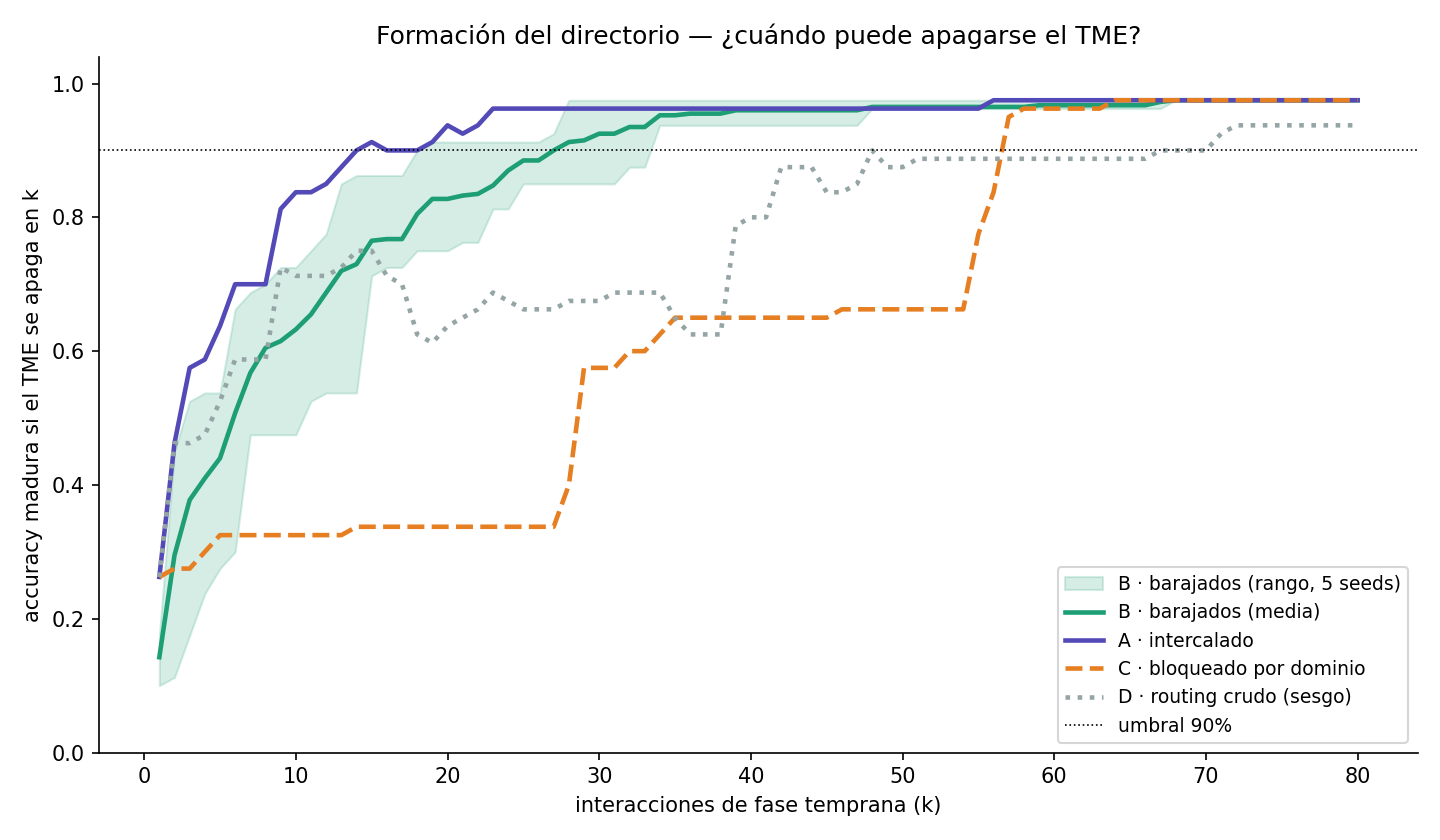
\includegraphics[width=0.92\textwidth]{formacion_directorio.png}
    \caption{Precisión madura en función del número de interacciones $k$ para
    las cuatro condiciones de formación. La línea punteada marca el umbral del
    90\,\%.}
    \label{fig:formacion}
\end{figure}

\paragraph{Capacidad y especificidad.}
Se probaron cinco valores de $N$: 25, 50, 100, 200 y 328 imágenes por clase.
La generalización sobre imágenes de test crece con la cobertura del llenado:
56.7\,\% en $N{=}200$ y 78.3\,\% en $N{=}328$.
La tasa de falsos aceptados fue de \textbf{0\,\% en todo el rango}: el containment
inverso con $\xi = 0$ nunca acepta una imagen de otra clase.
El enrutamiento de labels alcanza su mejor zona en $N = 200$ (97.5\,\%) y se degrada
en $N = 328$ (85.0\,\%) por saturación del eje contrario; por eso la zona de
operación recomendada es $N = 200$.

\paragraph{Calibración del directorio: por qué B1.}
Se compararon nueve condiciones de lectura del directorio
(Tabla~\ref{tab:calibracion}).
B1 es la que ataca el mecanismo causal: convertir activación acumulada en
evidencia por interacción. Por eso domina; las demás manipulan síntomas
(el vocabulario con F, el sesgo de consultas con D, el cap de registros con C)
sin tocar la raíz.

\begin{table}[H]
    \centering
    \caption{Precisión madura bajo distintas condiciones de lectura del
    directorio ($N = 80$).}
    \label{tab:calibracion}
    \small
    \begin{tabular}{llc}
        \toprule
        Condición & Descripción & Precisión (\%) \\
        \midrule
        A (cruda)     & Score de activación sin normalizar               & 53.75 \\
        B1            & División entre conteo de registros por agente     & \textbf{98.75} \\
        B2            & División entre raíz cuadrada del conteo           & 75.00 \\
        C             & Cap de número máximo de registros por agente      & 53.75 \\
        D             & Consultas balanceadas entre clases                & 52.82 \\
        E32 / E64     & Cuantización binaria en 32 / 64 niveles           & 53.75 \\
        F             & Vocabulario curado (sin ruido Apple Inc.)         & 80.00 \\
        G (D+B1+F)    & Consultas balanceadas + B1 + vocabulario curado   & 98.72 \\
        \bottomrule
    \end{tabular}
\end{table}

\begin{figure}[H]
    \centering
    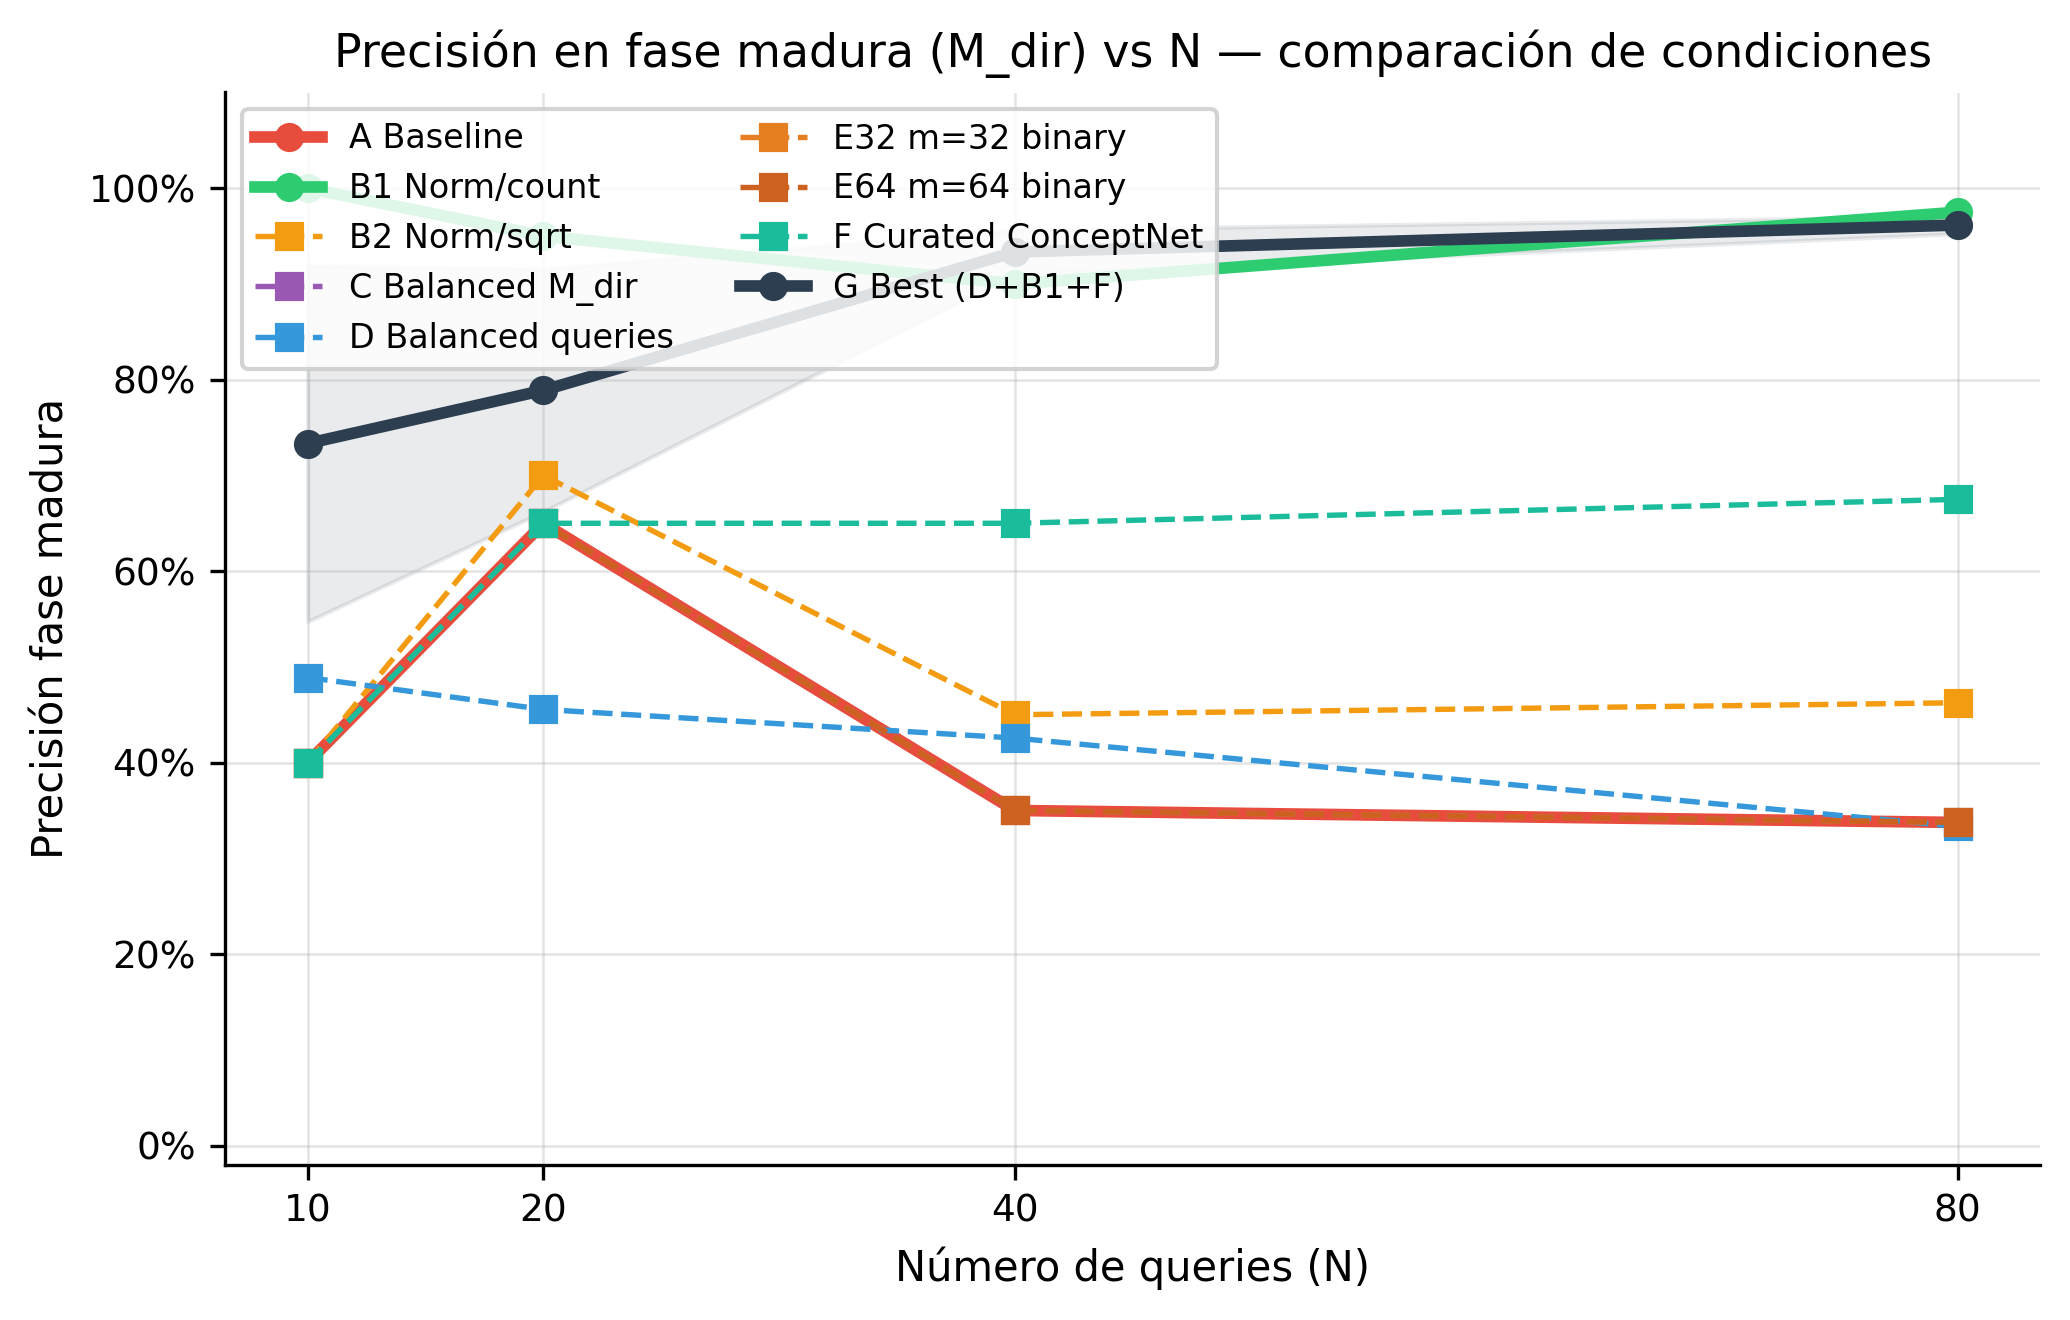
\includegraphics[width=0.92\textwidth]{ablation_madura.png}
    \caption{Precisión madura en función de $N$ para cada condición de lectura.
    Solo B1 (y su combinación G) sostienen precisión alta en todo el rango.}
    \label{fig:ablation}
\end{figure}

\paragraph{Hemisferio visual e inversa.}
En la dirección imagen $\to$ palabras, el enrutamiento visual acierta el
\textbf{100\,\%} de las imágenes que acepta (la cobertura con $\xi = 0$ es la
restricción: 32.9\,\% del test) y la evocación de dominio top-3 alcanza
\textbf{16/17 = 94.1\,\%}.
En la dirección texto $\to$ imagen, las recuperaciones visuales deben leerse como
imágenes prototípicas del dominio, producidas por la acumulación de registros
en la memoria y no como copias de imágenes particulares.

\begin{figure}[H]
    \centering
    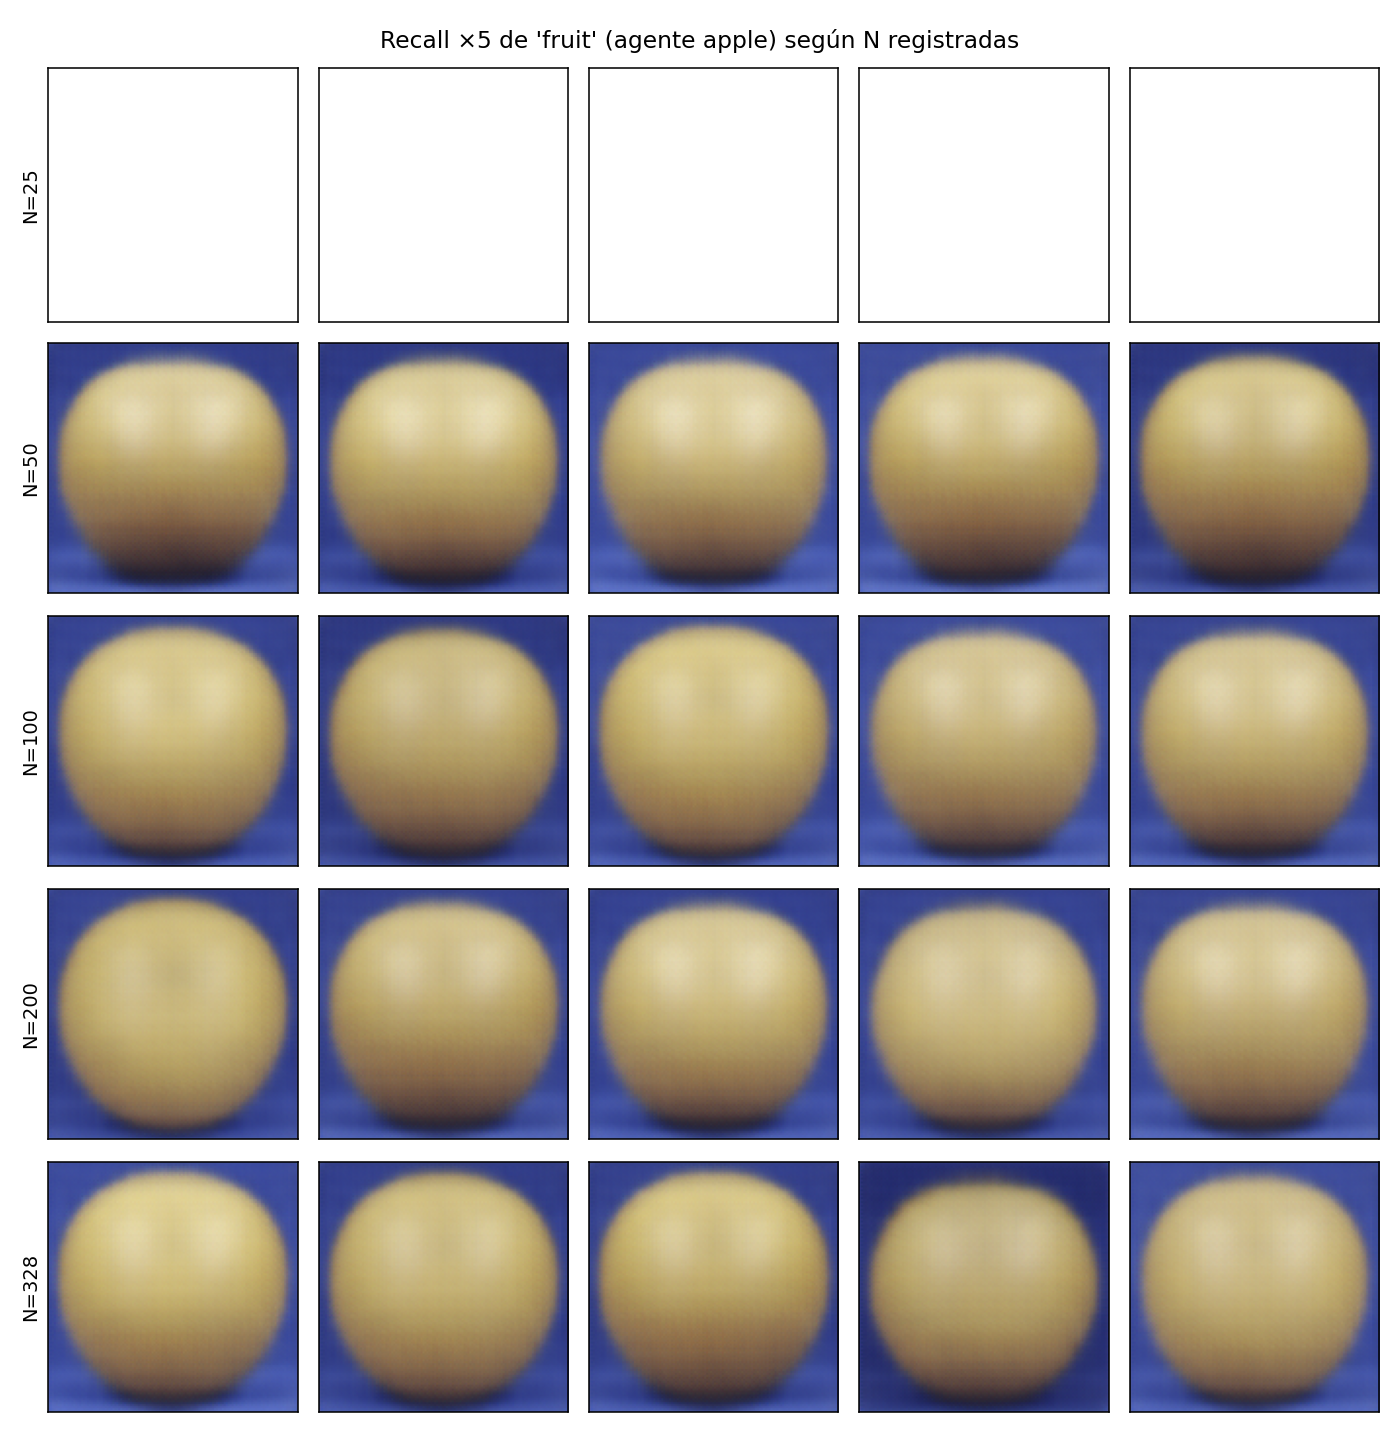
\includegraphics[width=0.92\textwidth]{recall_por_n.png}
    \caption{Imágenes recuperadas para la consulta ``fruit'' con distintos
    tamaños de llenado $N$. A mayor cobertura, la memoria produce recuperaciones con
    más variedad; cada imagen recuperada es prototípica porque surge de la
    distribución acumulada en la memoria.}
    \label{fig:recall-por-n}
\end{figure}

\paragraph{El hallazgo de fondo: el sesgo venía del llenado.}
El sesgo de densidad que motivó varias calibraciones externas no era un defecto
de la EAM sino una consecuencia de llenar mal las memorias.
Con un prototipo promedio repetido $N$ veces, la recuperación colapsa a un solo
patrón (variedad $L_1 = 0.00$); con instancias reales, 12 muestras producen
12 patrones distintos y las masas quedan igualadas por construcción.
La teoría de Pineda y Morales estaba completa: bastaba alimentarla con los
datos que el modelo requiere.
La forma en que se llena la memoria pesa más en el comportamiento del sistema
que cualquier ajuste posterior de parámetros.

% -------------------------------------------------------
\section{Limitaciones}

La cuantización por signo de fastText descarta la magnitud de los componentes.
Esto reduce el margen entre clases en el espacio semántico binario y puede
mezclar vocabularios cercanos, como ocurre con el caso polisémico de
\textit{apple}.

En el hemisferio visual, el uso de $\xi = 0$ mantiene una especificidad perfecta,
pero limita la cobertura: el sistema solo acepta imágenes suficientemente
similares a las ya registradas.
Además, las imágenes recuperadas dependen del decoder del autoencoder, por lo
que pueden verse suaves o con poco detalle de alta frecuencia.

Otra limitación importante es que, después de formar el directorio, los agentes
ya no siguen almacenando nuevos labels, imágenes o asociaciones.
La fase madura enruta y recupera con lo aprendido, pero no cubre todavía
procesos de aprendizaje continuo como \emph{transactive encoding} o
\emph{transactive retrieval}.

% -------------------------------------------------------
\section{Cierre}

Las Memorias Asociativas Entrópicas son una base suficiente para construir un
sistema de memoria transactiva multi-agente funcional, bidireccional
(texto $\leftrightarrow$ imagen) y con rechazo controlado, sin recurrir a
aprendizaje profundo supervisado para la toma de decisiones.
El directorio de Wegner emerge por interacción: rápido cuando la exposición
es variada y lento cuando se segrega por dominio. La única normalización
necesaria (B1) se deriva analíticamente de la definición de la proyección
hetero-asociativa.
Los siguientes pasos incluyen el barrido de $\xi > 0$, el uso de magnitudes de
fastText, el aprendizaje en fase madura y la rotación de miembros.

% -------------------------------------------------------
\bibliographystyle{apalike}
\bibliography{referencias}

\end{document}
